\section{Linear Regression}\label{sec:linear-regression}
\framecard{\insertsection}
\subsection{Defining models}

\begin{frame}{\insertsubsection}
	\framesubtitle{An initial curve fitting problem}

\begin{itemize}
	\item If we have a set of points in a space that comes from observations of an experiment and we want to predict other points, this could be done with \textbf{\textcolor{UniOrange}{curve fitting}}.
	\item So we could define some strategy to find our model.
\end{itemize}

\begin{block}{Strategy}
	\begin{itemize}
		\item[1] Purpose a \textcolor{UniBlue}{\textbf{model}}, e.g. functions like exponential, polynomial and others.
		\item[2] Train our model with the training data set, finding the \textcolor{UniBlue}{\textbf{unknown parameters}} or \textcolor{UniBlue}{\textbf{weights}}.
	\end{itemize}
\end{block}
\end{frame}


\begin{frame}{\insertsubsection}
	\framesubtitle{An initial curve fitting problem}
	\begin{itemize}
		\item Let's take the points below generated from the function $y(x)=\sin (2\pi x)$ with addition of Gaussian noise with zero mean and $0.2$ of standard deviation.
	\end{itemize}

	\begin{figure}
	\label{fig:plot-fitting-example}
		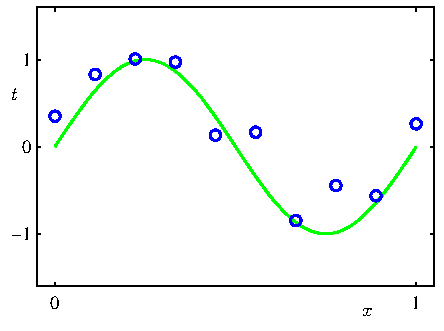
\includegraphics[totalheight=0.75\textheight]{Figure1c2.pdf}
	\end{figure}
\end{frame}

\begin{frame}{\insertsubsection}
	\framesubtitle{Chosing a model}
	\begin{itemize}
		\item We can express the curve with a polynomial, being the \textcolor{UniOrange}{\textbf{model}}
		\begin{align*}
			y(x,\mathbf{w}) &= w_0x^0 + w_1x^1 + w_2x^2  + ... + w_{M-1}x^{M-1}  = \sum^{M-1}_{j=1} w_j x^j
		\end{align*}	
		\item In general, we could write this \textcolor{UniOrange}{\textbf{weighted sum}} with any other function. In other words, we can put this in terms of $\phi_n(x)=x^n$, where $\phi$ could be other \textcolor{UniOrange}{\textbf{basis function}}.
		\item e.g. we could have different $y(x)$ for different basis functions, or \textcolor{UniOrange}{\textbf{features}}.
		\begin{align*}
			y(x,\mathbf{w}) &= w_0 \phi_0(x) +w_1 \phi_1(x) +w_2 \phi_2(x)  + ... + w_{M-1} \phi_{M-1}(x) \\
							&= w_0 \exp\left\{ - \frac{(x-\mu_0)^2}{2\sigma^2}\right\} + w_1  \exp\left\{ - \frac{(x-\mu_1)^2}{2\sigma^2}\right\} + \\ & ... + w_{M-1} \exp\left\{ - \frac{(x-\mu_{M-1})^2}{2\sigma^2}\right\} \\
							&= w_0 \sin(0 \cdot x) + w_1 \cos(1 \cdot x) + \\ &... + w_{M_2} \sin((M-2) \cdot x) + w_{M-1} \cos((M-1) \cdot x)
		\end{align*}

\end{itemize}
\end{frame}

\begin{frame}{\insertsubsection}
	\framesubtitle{A non-linear model linear in parameters}
	\begin{columns}
		\begin{column}{0.475\textwidth}
			\begin{itemize}
				\item For simplicity, we'll carry this notation along.
				\begin{align*}
					y(x,\mathbf{w}) &= w_0 \phi_0(x) +w_1 \phi_1(x) + ...\\
					& + w_{M-1} \phi_{M-1}(x) \\
									&= \sum^{M-1}_{j=1} w_j \phi_j(x)
				\end{align*}
				\item We'll evaluate $\phi$ for all $x$, and then project it in the $w$ vector space, the \textbf{\textcolor{UniOrange}{feature-space}}, then our model could be formed by \textcolor{UniOrange}{\textbf{non-linear}} functions. But, remaining \textcolor{UniOrange}{\textbf{linear on parameters}}.
			\end{itemize}
		\end{column}
		\begin{column}{0.475\textwidth}  
			\begin{center}
			\centering
			\includegraphics[totalheight=0.6\textwidth]{{Figure3.2}}
			 \end{center}
		\end{column}
		\end{columns}
\end{frame}
%%%%%%%%%%%%%%%%%%%%%%%%%%%%%%%%%%%%%%%%%%%%%%%%%%%%%%%%%

\subsection{Optimizing the parameters}

%%%%%%%%%%%%%%%%%%%%%%%%%%%%%%%%%%%%%%%%%%%%%%%%%%%%%%%%%
\begin{frame}{\insertsubsection}
	\framesubtitle{The model parameters}
\begin{columns}
\begin{column}{0.475\textwidth}
	\begin{itemize}
		\item The chosen model will give us some curve that is needed to adjust such that we'll \textcolor{UniOrange}{\textbf{minimize its distance}} to the \textcolor{UniOrange}{\textbf{targets}} $t$.
		\item This approach lead us to use the \textcolor{UniOrange}{\textbf{least squares}} to estimate the weights and minimize the \textcolor{UniOrange}{\textbf{error}} $E$.
		\begin{align*}
			E(\mathbf{w}) \triangleq \frac{1}{2} \sum_{n=1}^N \left\{ y_n -  t_n \right\}^2
		\end{align*}
	\end{itemize}
\end{column}
\begin{column}{0.475\textwidth}  
    \begin{center}
	\centering
	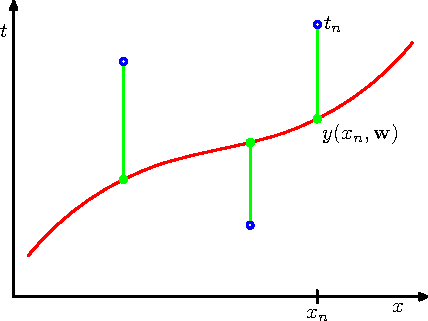
\includegraphics[totalheight=0.4\textheight]{Figure1c3.pdf}
     \end{center}
\end{column}
\end{columns}

\end{frame}
%%%%%%%%%%%%%%%%%%%%%%%%%%%%%%%%%%%
%\begin{frame}{\insertsubsection}

%\textcolor{red}{Insert some \textit{Minkowski} loss.}

%\end{frame}
%%%%%%%%%%%%%%%%%%%%%%%%%%%%%%%%
\begin{frame}{\insertsubsection}
	\framesubtitle{The model parameters}
	\textcolor{UniGold}{\textbf{Why choose a quadratic norm distance?}}
	\begin{figure}
    \begin{subfigure}[t]{0.5\textwidth}
        \centering
        \includegraphics[totalheight=0.35\textheight]{"Figure1.29a".eps}
    \end{subfigure}%
    \begin{subfigure}[t]{0.5\textwidth}
        \centering
        \includegraphics[totalheight=0.35\textheight]{"Figure1.29b".eps}
		\end{subfigure}
		\\
	\begin{subfigure}[t]{0.5\textwidth}
		\centering
		\includegraphics[totalheight=0.35\textheight]{"Figure1.29c".eps}
	\end{subfigure}%
	\begin{subfigure}[t]{0.5\textwidth}
		\centering
		\includegraphics[totalheight=0.35\textheight]{"Figure1.29d".eps}
	\end{subfigure}
	\end{figure}
\end{frame}

\begin{frame}{\insertsubsection}
	\framesubtitle{The model parameters}
	\textcolor{UniGold}{\textbf{Why choose a quadratic norm distance?}}\footnote{See Appendix ?}
	\begin{itemize}
		\item The first row figures could be used for the derivations, taking care with some \textcolor{UniOrange}{\textbf{non-continuous derivatives}}.
		\item We'll use the \textcolor{UniOrange}{\textbf{quadratic norm}} because its the minor integer $q$ differentiable, and then the error measures $E$ between the model $y(x,\mathbf{w})$ and the targets $t$ will be euclidean.
		\item More, increasing the value of $q$, the smallests than 1 and bigger than 0 errors between the model and the targets that become irrelevant for $E$.
	\end{itemize}
\end{frame}

\begin{frame}{\insertsubsection}
	\framesubtitle{Matrix form}
	\begin{itemize}
		\item Remembering that
			\begin{align*}
				y(x,\mathbf{w}) &= w_0 \phi_0(x) +w_1 \phi_1(x) +w_2 \phi_2(x)  + ... + w_{M-1} \phi_{M-1}(x) 
			\end{align*}
		\item We'll evaluate for all $x_i$ values, and then put $y_n(x_i,\mathbf{w})$ in the matrix form and get
		\begin{equation*}
			y_n=
			\begin{bmatrix}
				\phi_0(x_n) & \phi_1(x_n) & ... & \phi_{M-1}(x_n)
			\end{bmatrix}
			\begin{bmatrix}
				w_0 & w_1 &  \cdots & w_{M-1}
			\end{bmatrix}^{\top}
		\end{equation*}
		\item And then
		\begin{equation*}
			\underbrace{
				\begin{bmatrix}
				y_0 \\ y_1 \\  \vdots \\ y_{N-1}
				\end{bmatrix}
			}_\mathbf{y} = 
			\underbrace{
				\begin{bmatrix}
				\phi_0(x_0) & \phi_1(x_0) & ... & \phi_{M-1}(x_0)   \\ 
				\phi_0(x_1) & \phi_1(x_1) & ... & \phi_{M-1}(x_1)    \\ 
				\vdots & \vdots & \ddots & \vdots \\
				\phi_0(x_{N-1}) & \phi_1(x_{N-1}) & ... & \phi_{M-1}(x_{N-1})  
				\end{bmatrix}
			}_\Phi
			\underbrace{
				\begin{bmatrix}
				w_0 \\ w_1 \\  \vdots \\ w_{N-1}
				\end{bmatrix}
			}_\mathbf{w}
		\end{equation*}
		where $\Phi$ is the \textcolor{UniOrange}{\textbf{design matrix}}.
		\item This represents the system $\mathbf{y} = \Phi \mathbf{w}$.
\end{itemize}
\end{frame}

\begin{frame}{\insertsubsection}
	\framesubtitle{The cost function and minimization problem}
	\begin{itemize}
		\item If $E(\mathbf{w}) = \frac{1}{2} \left( \mathbf{y} - \mathbf{t} \right)^{\top}\left( \mathbf{y} - \mathbf{t} \right)$ where $\mathbf{t} = \begin{bmatrix} t_1 & t_2 & ... & t_n
		\end{bmatrix}^{\top}$
		\item Then we'll have 
		\begin{align*}
			E(\mathbf{w}) &= \frac{1}{2} \left( \mathbf{y}^{\top}\mathbf{y} -  \mathbf{t}^{\top}\mathbf{y} - \mathbf{y}^{\top}\mathbf{t} + \mathbf{t}^{\top}\mathbf{t} \right) \\
					   &= \frac{1}{2} \left( ( \Phi \mathbf{w})^{\top}( \Phi \mathbf{w}) -  \mathbf{t}^{\top}( \Phi \mathbf{w}) - ( \Phi \mathbf{w})^{\top}\mathbf{t} + \mathbf{t}^{\top}\mathbf{t} \right) \\
					   &= \frac{1}{2} \left( \mathbf{w}^{\top} \Phi^{\top} \Phi \mathbf{w} -  2\mathbf{t}^{\top} \Phi \mathbf{w} + \mathbf{t}^{\top}\mathbf{t} \right)
		\end{align*}
		\item In sequence, we'll try to minimize it in terms of the weights ($\mathbf{w}$) by
			\begin{align*}
				0 &= \frac{\partial E(\mathbf{w})}{\partial \mathbf{w}} = \frac{1}{2} \left( 2 \mathbf{w}^{\top} \Phi^{\top} \Phi  -  2\mathbf{t}^{\top} \Phi + 0 \right) \\
				\mathbf{w}^{\top} &=  \mathbf{t}^{\top} \Phi \left( \Phi^{\top} \Phi \right)^{-1} \\
				\mathbf{w}^* &= \left( \Phi^{\top} \Phi \right)^{-1}\Phi^{\top} \mathbf{t}
			\end{align*}
		\item Here, we've obtained the weights $\mathbf{w}^*$ with the \textcolor{UniOrange}{\textbf{best fit}} of the curve.
		\item We could say that the model \textcolor{UniOrange}{\textbf{learned}} the parameters.
		% \item Then too, $E(\mathbf{w})$	 remains scalar.
	\end{itemize}
\end{frame}

%\begin{frame}
% \vspace{1em}
%\lstinputlisting[linerange={3-7,11-12,14-15,17-17,23-23}]{codes/lnReg.m}
%\end{frame}

\begin{frame}{\insertsubsection}
	\framesubtitle{The over-fitting phenomenon}
	\textcolor{UniGold}{\textbf{Why the prediction is so distant from the deterministic curve?}}
	\begin{columns}
		\begin{column}{0.475\textwidth}
			\begin{itemize}	
			\item A visible effect of the \textcolor{UniOrange}{\textbf{increase of the complexity}} of the model, is the increase of the \textcolor{UniOrange}{\textbf{number of features}} $M$.
			\item It's easy to see that our model start's to differ from the $y$ and starts to interpolate the noise. We call this of \textcolor{UniOrange}{\textbf{over-fitting}}.
			\item This phenomenon illustrate a method of always search for the \textcolor{UniOrange}{\textbf{best estimation of the parameters}}.
			
			\vspace{1em}
			
			\end{itemize}
		\end{column}
		\begin{column}{0.475\textwidth}  %%<--- here
			\begin{animateinline}[autoplay,loop]{5}
				%  \input{./codes/lnReg/"lnReg_frame_1"}\newframe
				%  \input{./codes/lnReg/"lnReg_frame_2"}\newframe
				%  \input{./codes/lnReg/"lnReg_frame_3"}\newframe
				%  \input{./codes/lnReg/"lnReg_frame_4"}\newframe
				%  \input{./codes/lnReg/"lnReg_frame_5"}\newframe
				%  \input{./codes/lnReg/"lnReg_frame_6"}\newframe
				%  \input{./codes/lnReg/"lnReg_frame_7"}\newframe
				%  \input{./codes/lnReg/"lnReg_frame_8"}\newframe
				%  \input{./codes/lnReg/"lnReg_frame_9"}\newframe
				  \input{./codes/lnReg/"lnReg_frame_10"}\newframe
				%  \input{./codes/lnReg/"lnReg_frame_11"}\newframe
				%  \input{./codes/lnReg/"lnReg_frame_12"}\newframe
				%  \input{./codes/lnReg/"lnReg_frame_13"}\newframe
				%  \input{./codes/lnReg/"lnReg_frame_14"}\newframe
				%  \input{./codes/lnReg/"lnReg_frame_15"}\newframe
				%  \input{./codes/lnReg/"lnReg_frame_16"}\newframe
				%  \input{./codes/lnReg/"lnReg_frame_17"}\newframe
				%  \input{./codes/lnReg/"lnReg_frame_18"}\newframe
				%  \input{./codes/lnReg/"lnReg_frame_19"}\newframe
				% \input{./codes/lnReg/"lnReg_frame_20"}
			 \end{animateinline}
		\end{column}
	\end{columns}
\end{frame}


\begin{frame}{\insertsubsection}
	\framesubtitle{Training and testing}
	\textcolor{UniGold}{\textbf{Could be over-fitting a problem?}}
	\begin{columns}
		\begin{column}{0.475\textwidth}
			\begin{itemize}	
			\item We could \textcolor{UniOrange}{\textbf{train}} our model, it means evaluate $\mathbf{w}^*$, for only a part of our dataset.
			\item If the model be a good one, the error must be small when its \textcolor{UniOrange}{\textbf{testing}}, i.e. the error must be small when we evaluate all dataset with the $\mathbf{w}^*$ of the trained part.
			\item But this in general does not occur and the \textcolor{UniOrange}{\textbf{error increases}}.
			\end{itemize}
		\end{column}
		\begin{column}{0.475\textwidth}  %%<--- here
			\begin{center}
			\centering
			\label{fig:Erms}
			\includegraphics[width=1\linewidth]{"Figure1.5".eps}
			\end{center}
		\end{column}
	\end{columns}		
	\end{frame}

\begin{frame}{\insertsubsection}
	\framesubtitle{Regularizing the parameters}
	\textcolor{UniGold}{\textbf{How to control the over-fitting?}}
	\begin{columns}
		\begin{column}{0.475\textwidth}
			\begin{itemize}	
			\item With the increase of the model complexity, the value of $\mathbf{w}^*$ increases too.
			\item A solution could be add a \textcolor{UniOrange}{\textbf{penalty term}} as the norm of the weights increases.
			\item To control the over-fitting, we try to \textcolor{UniOrange}{\textbf{regularize}} the weights by adding a penalty term $\lambda$ to error function, by this we force the coefficients to not reach high values.
			\begin{align*}
				\tilde{E}(\mathbf{w}) &=\frac{1}{2} (\mathbf{y}-\mathbf{t})^{\top}(\mathbf{y}-\mathbf{t}) +\frac{\lambda}{2} \mathbf{w}^{\top}\mathbf{w} \\
		\Rightarrow & \mathbf{w}^*_\text{reg} = \left( \Phi^{\top} \Phi + \lambda \mathbf{I} \right)^{-1} \Phi^{\top} \mathbf{t}
	\end{align*}			
			\end{itemize}
		\end{column}
		\begin{column}{0.475\textwidth}  %%<--- here
			\centering
			% \begin{figure}
			% 	\setlength\fwidth{0.075\textwidth}
			% 	\input{./codes/"lnReg-Wmod".tex}
			% \end{figure}
			%\begin{center}
			%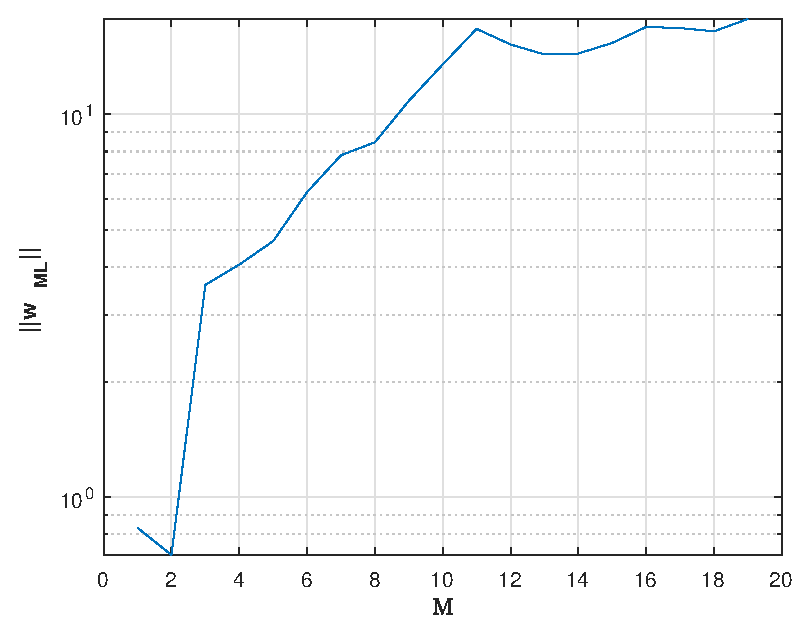
\includegraphics[width=1\linewidth]{lnReg-Wmod.eps}
			%\end{center}
			\begin{animateinline}[autoplay,loop]{5}
				%  \input{./codes/lnRegRegulated/"lnRegRegulated_frame_1"}\newframe
				%  \input{./codes/lnRegRegulated/"lnRegRegulated_frame_2"}\newframe
				%  \input{./codes/lnRegRegulated/"lnRegRegulated_frame_3"}\newframe
				%  \input{./codes/lnRegRegulated/"lnRegRegulated_frame_4"}\newframe
				%  \input{./codes/lnRegRegulated/"lnRegRegulated_frame_5"}\newframe
				%  \input{./codes/lnRegRegulated/"lnRegRegulated_frame_6"}\newframe
				%  \input{./codes/lnRegRegulated/"lnRegRegulated_frame_7"}\newframe
				%  \input{./codes/lnRegRegulated/"lnRegRegulated_frame_8"}\newframe
				%  \input{./codes/lnRegRegulated/"lnRegRegulated_frame_9"}\newframe
				%  \input{./codes/lnRegRegulated/"lnRegRegulated_frame_10"}\newframe
				%  \input{./codes/lnRegRegulated/"lnRegRegulated_frame_11"}\newframe
				%  \input{./codes/lnRegRegulated/"lnRegRegulated_frame_12"}\newframe
				%  \input{./codes/lnRegRegulated/"lnRegRegulated_frame_13"}\newframe
				%  \input{./codes/lnRegRegulated/"lnRegRegulated_frame_14"}\newframe
				%  \input{./codes/lnRegRegulated/"lnRegRegulated_frame_15"}\newframe
				%  \input{./codes/lnRegRegulated/"lnRegRegulated_frame_16"}\newframe
				%  \input{./codes/lnRegRegulated/"lnRegRegulated_frame_17"}\newframe
				%  \input{./codes/lnRegRegulated/"lnRegRegulated_frame_18"}\newframe
				%  \input{./codes/lnRegRegulated/"lnRegRegulated_frame_19"}\newframe
				\input{./codes/lnRegRegulated/"lnRegRegulated_frame_100"}\newframe
			 \end{animateinline}
		\end{column}
	\end{columns}
\end{frame}

\begin{frame}{\insertsubsection}
	\framesubtitle{Regularizing the parameters}
	\textcolor{UniGold}{\textbf{How to control the over-fitting?}}
	\begin{columns}
		\begin{column}{0.475\textwidth}
			\begin{itemize}	
			\item With the increase of the model complexity, the value of $\mathbf{w}^*$ increases too.
			\item A solution could be add a \textcolor{UniOrange}{\textbf{penalty term}} as the norm of the weights increases.
			\item To control the over-fitting, we try to \textcolor{UniOrange}{\textbf{regularize}} the weights by adding a penalty term $\lambda$ to error function, by this we force the coefficients to not reach high values.
			\begin{align*}
				\tilde{E}(\mathbf{w}) &=\frac{1}{2} (\mathbf{y}-\mathbf{t})^{\top}(\mathbf{y}-\mathbf{t}) +\frac{\lambda}{2} \mathbf{w}^{\top}\mathbf{w} \\
		\Rightarrow & \mathbf{w}^*_\text{reg} = \left( \Phi^{\top} \Phi + \lambda \mathbf{I} \right)^{-1} \Phi^{\top} \mathbf{t}
	\end{align*}			
			\end{itemize}
		\end{column}
		\begin{column}{0.475\textwidth}  %%<--- here
			\centering
			\includegraphics[width=1\linewidth]{"Figure1.8"}
		\end{column}
	\end{columns}
\end{frame}


% \begin{frame}{\insertsubsection}
% 	\framesubtitle{Regularizing the parameters}
% 		\begin{itemize}
% 		\item To control the over-fitting, we try to \textcolor{UniOrange}{\textbf{regularize}} the weights by adding a penalty term $\lambda$ to error function, by this we force the coefficients to not reach high values.

		
% 				\begin{align*}
% 					\tilde{E}(\mathbf{w}) &=\frac{1}{2} (\mathbf{y}-\mathbf{t})^{\top}(\mathbf{y}-\mathbf{t}) +\frac{\lambda}{2} \mathbf{w}^{\top}\mathbf{w} \\
% 									   &= \frac{1}{2} \left( \mathbf{w}^{\top} \Phi^{\top} \Phi \mathbf{w} -  2\mathbf{t}^{\top} \Phi \mathbf{w} + \mathbf{t}^{\top}\mathbf{t} + \lambda \mathbf{w}^{\top}\mathbf{I}\mathbf{w} \right) \\
% 			\Rightarrow \frac{\partial E(\mathbf{w})}{\partial \mathbf{w}} &= \frac{1}{2} \left( 2 \mathbf{w}^{\top} \Phi^{\top} \Phi  -  2\mathbf{t}^{\top} \Phi + 0 + 2 \lambda \mathbf{w}^{\top} \mathbf{I} \right) \\
% 					0 &=  \mathbf{w}^{\top} \Phi^{\top} \Phi  -  \mathbf{t}^{\top} \Phi + \lambda \mathbf{w}^{\top} \mathbf{I} \\
% 					 \mathbf{w}^*_\text{reg} = & \left( \Phi^{\top} \Phi + \lambda \mathbf{I} \right)^{-1} \Phi^{\top} \mathbf{t}
% 		\end{align*}			
% 		\end{itemize}
% \end{frame}

%\begin{frame}
	% \vspace{1em}
%	\lstinputlisting[linerange={3-7,12-16,18-18,24-24}]{codes/lnRegRegulated.m}
%\end{frame}


% \begin{frame}{\insertsubsection}
% 	\framesubtitle{Training and testing}
% 	\textcolor{UniGold}{\textbf{A more sophisticated approach?}}
% 	\begin{columns}
% 		\begin{column}{0.475\textwidth}
% 			\begin{itemize}	
% 			\item We could \textcolor{UniOrange}{\textbf{train and test}} and evaluate the error for several values of $\lambda$.
% 			\item Even yet, it's too wasteful partitionate and optimize data to find good model parameters or even a \textcolor{UniOrange}{\textbf{flexible}} one.
% 			\item We need a more sophisticated approach.
% 			\end{itemize}
% 		\end{column}
% 		\begin{column}{0.475\textwidth}
% 			\begin{center}
% 			\centering
% 			\label{fig:Erms-reg}
% 			\includegraphics[width=1\linewidth]{"Figure1.8".eps}
% 			\end{center}
% 		\end{column}
% 	\end{columns}		
% 	\end{frame}

%%%%%%%%%%%%%%%%%%%%%%%%%%%%%%%%%%%%%%%%%%%%%%%%%%

\subsection{An uncertainty perspective}

%%%%%%%%%%%%%%%%%%%%%%%%%%%%%%%%%%%%%%%%%%%%%%%%%%

\begin{frame}{\insertsubsection}
	\framesubtitle{Looking back the regression}
	\textcolor{UniGold}{\textbf{What if we assume not knowing the data exactly?}}
	\begin{columns}
	\begin{column}{0.475\textwidth}
		\begin{itemize}
			\item Having an \textcolor{UniOrange}{\textbf{uncertainty}} in the measured value, we could represent it with a \textcolor{UniOrange}{\textbf{probability distribuition}}.
			\item Now, each \textcolor{UniOrange}{\textbf{target}} could be expressed as a \textcolor{UniOrange}{\textbf{random variable}}.
			\item Its \textcolor{UniOrange}{\textbf{mean}} is given by $y(x,\mathbf{w})$, and the \textcolor{UniOrange}{\textbf{variance}} by $1/\sigma^2 = \beta$.
			\item $\beta$ is known as \textcolor{UniOrange}{\textbf{precision parameter}} too.
		\end{itemize}
		\end{column}
		\begin{column}{0.475\textwidth}  %%<--- here
			\begin{center}
				\includegraphics[width=1\linewidth]{"Figure1.16"}
			\end{center}
		\end{column}
	\end{columns}
\end{frame}


\begin{frame}{\insertsubsection}	
	\framesubtitle{Targets as distributions}
	\begin{itemize}
		\item Being the random variables independent and identically distributed, we can say that our \textcolor{UniOrange}{\textbf{joint probability}} is given by
	\begin{equation*}
		p(\mathbf{t} | \mathbf{x}, \mathbf{w}, \beta) = \prod_{n=1}^N p \left( t_n | x_n, \mathbf{w}, \beta \right)
	\end{equation*}
		\item Our goal is, given the \textcolor{UniOrange}{\textbf{parameters}} $\mathbf{w}$, maximize the \textcolor{UniOrange}{\textbf{probability}} of the \textcolor{UniOrange}{\textbf{targets}}.
		\item  Before, consider a property of the probability distribuitions
		\begin{equation*}
		\int_\infty ^{-\infty} p(x) dx = 1 \text{ and } p(x) \geq 0
		\end{equation*}
		\item Then, to avoid computational singularity and obtain a monotonically increasing function, we apply
		\begin{equation*}
			\ln \left( p( \mathbf{t}| \mathbf{x}, \mathbf{w}, \beta) \right) = \sum_{n=1}^N \ln \left(   p \left( t_n | x_n, \mathbf{w}, \beta \right) \right)
		\end{equation*}		
	\end{itemize}
\end{frame}

% \begin{frame}{\insertsubsection}
% 	\framesubtitle{But which distribuition choose?}
% 	\begin{columns}
% 		\begin{column}{0.475\textwidth}
% 			\begin{itemize}
% 				\item We'll choose the \textcolor{UniOrange}{\textbf{Gaussian distribution}} just for convenience.
% 				\item Then we can state the distribution for each target and then
% 				\begin{equation*}
% 					p( t| \mathbf{x}, \mathbf{w}, \beta) = \mathcal{N} \left( t | y(\mathbf{x}, \mathbf{w}), \beta^{-1} \right)
% 				\end{equation*}
% 				\item And we'll try to \textcolor{UniOrange}{\textbf{maximize}}	the targets probability.
% 			\end{itemize}
% 		\end{column}
% 		\begin{column}{0.475\textwidth}
% 			\includegraphics[width=1\linewidth]{"Figure1.13".pdf}
% 		\end{column}
% 	\end{columns}
% 	\begin{block}{One-dimensional Gaussian distribution}
% 		\begin{equation*}
% 			\mathcal{N}(x | \mu, \sigma^2) = \frac{1}{(2 \pi \sigma^2)^{1/2}} \exp \left\{ -\frac{1}{2 \sigma^2} (x- \mu)^2 \right\} > 0
% 		\end{equation*}
% 		where $\mu$ is the mean and $\sigma^2$ the variance.
% 	\end{block}	
% \end{frame}

\begin{frame}{\insertsubsection}
	\framesubtitle{Back to the cost function}
	\begin{itemize}
		\item From the \textcolor{UniOrange}{\textbf{joint probability}} of the Gaussians distributions we have
		\begin{align*}
				\ln \left( p( \mathbf{t}| \mathbf{x}, \mathbf{w}, \beta) \right) 
				&= \mathcal{N} \left( t | y(\mathbf{x}, \mathbf{w}), \beta^{-1} \right) \\
				&= \sum_{n=1}^N - \frac{1}{2} \ln (2 \pi) + \sum_{n=1}^N \frac{1}{2} \ln \beta - \sum_{n=1}^N \frac{\beta}{2} (x_n -  y(x_n, \mathbf{w}))^2
		\end{align*}
		\item If we make
		\begin{align*}
			\frac{\partial}{\partial \mathbf{w}}\ln \left( p( \mathbf{t}| \mathbf{x}, \mathbf{w}, \beta) \right) = 0
		\end{align*}
		we'll obtain the \textcolor{UniOrange}{\textbf{cost function}} obtained before in the linear regression, then our assumptions are well grounded.
		\item With the maximization, we'll obtain the weights $\mathbf{w}$ that \textcolor{UniOrange}{\textbf{maximize}} the log probability of the targets, given the parameters.
		%\item With this approach, we expect to obtain too the same \textcolor{UniOrange}{\textbf{over-fitting}} problem.\footnote{See Appendix ?}
		\item This is called \textcolor{UniOrange}{\textbf{maximum likelihood}}, since we are looking for the \textcolor{UniOrange}{\textbf{parameters}} distribution that are more probable to had been generated the data.
		\item This is a initial step towards to a \textcolor{UniOrange}{\textbf{Bayesian}} approach.
	\end{itemize}
\end{frame}